\chapter{Conclusion and Direction of Further Work} \label{ch:WorkDirection}

\section{Synthesis of Ideas and Discussion}
As indicated in \cref{Intro}, a hollow-core PCF can be thought of as a periodic, thin-structure material occupying a fixed domain.
We can represent this mathematically using a domain $\homDomain$ with holes, which we interpret as inclusions (of the solid-core material) or as vacuum (hollow-core) - for simplicity we will discuss the hollow-core case.
Then we are interested in determining which frequencies of light will be trapped by the fibre, due to the choice of PCF material and geometry of $\homDomain$.
We will use the system of Maxwell equations,
\begin{align} \label{eq:MaxwellSystem}
	\grad\wedge\mathbf{E} = \pdiff{t}\bracs{\magP \mathbf{H}}, &\quad
	\grad\wedge\mathbf{H} = -\pdiff{t}\bracs{\elcP \mathbf{E}},
\end{align}
as the basis for this model; as before (\sref{PCFs}) denotes the electric $\mathbf{E}$ and magnetic $\mathbf{H}$ fields, $\elcP$ and $\magP$ the electric permittivity and magnetic permeability of the medium the light is propagating in.
This problem can be formulated in the homogenisation setting (\sref{FreqApproxes}) by identifying a suitable period cell and introducing appropriate length scales $\epsilon$ and $N$.
From \sref{AsymRegimes} we know that we can gain knowledge about the spectrum of a thin-structure problem from analysis of a related singular-structure problem (provided the appropriate vertex and edge scaling is accounted for), which is more often open to an analytic approach.
Therefore the design of the PCF (hence the domain $\homDomain$) admits some analysis of its spectrum, and so gain knowledge of the frequencies of light which the PCF is expected to trap.
Schematically this is illustrated in \fref{PhDModel}, and in what follows we will discuss extending the content of this report to the setting just described.
Note that since we are working with a finite domain with a large number of periods, it will be more appropriate to work in the high-frequency approximation during the following discussion.
Furthermore, in this section we assume we have a PCF design in the form of a periodic domain $\homDomain$  and the corresponding periodic graph $\graph$ (that arises from finding the corresponding singular structure).
We let $\homDomain_{N}$ and $\graph_{N}$ denote the high-frequency approximation domains for each $N\in\naturals$ (that is, the finite domain filled with $N$ copies of the unit cell stacked in each direction), see \sref{FreqApproxes}. 
\begin{figure}[b!]
	\centering
	\begin{tikzpicture}
		%domain part
		\filldraw[pattern=hexagons, draw=black] (0,0) circle (1);
		\draw[->] (1,-1) -- (2,-2);
		\node[anchor=south] at (0,1) {Proposed PCF structure};
		%singular structure part, graph that's periodic
		\draw (2.5,-2.5) -- (3.2,-2.5) -- (3.7,-3) -- (3.2,-3.5) -- (2.5,-3.5) -- (2,-3) -- cycle;
		\filldraw[color=black] (2.5,-2.5) circle (1.5pt);
		\filldraw[color=black] (3.2,-2.5) circle (1.5pt);
		\filldraw[color=black] (3.7,-3) circle (1.5pt);
		\filldraw[color=black] (3.2,-3.5) circle (1.5pt);
		\filldraw[color=black] (2.5,-3.5) circle (1.5pt);
		\filldraw[color=black] (2,-3) circle (1.5pt);
		\draw[->] (2,-4) -- (1,-5);
		\node[anchor=west, align=left] at (4,-3) {Periodic singular \\ structure problem};
		%band-gap spectrum part
		\draw (-1,-6) -- (1,-6);
		\draw[color=red, line width=2pt] (-0.9,-6) -- (-0.4,-6);
		\draw[color=red, line width=2pt] (0,-6) -- (0.3,-6);
		\draw[color=red, line width=2pt] (0.85,-6) -- (1,-6);
		\draw[->] (-1,-5) -- (-2,-4);
		\node[anchor=south] at (-0.65,-6) {$I_{1}$};
		\node[anchor=south] at (0.15,-6) {$I_{2}$};
		\node[anchor=south] at (0.925,-6) {$I_{3}$};
		\node[anchor=north, align=center] at (0,-6.2) {Analysis to determine \\ spectrum};
		%inform design part
		%\draw (-4,-4) rectangle (-2,-2);
		\node[align=center] at (-3,-3) {Determine \\ suitability  \\ for use as \\ PCF};
		\draw[->] (-2,-2) -- (-1,-1);
		\node[anchor=north west] at (-1.5,-1.5) {Redesign};
		\draw[->] (-3,-2) -- (-3,-1);
		\node[anchor=south] at (-3,-1) {Fabrication};
		%"reformulation" box
		\draw[dashed, color=red] (-2,-7.75) rectangle (7,1.75);
		\node[anchor=south east, align=right] at (7,-7.75) {Reformulation of \\ previous ideas. \\ Areas requiring \\ analysis.};
	\end{tikzpicture}
	\caption{A diagram to illustrate how the concepts and theory presented in the preceeding chapters can be turned into a model of PCFs. The dashed-red box contains the areas which future work will focus on.\label{fig:PhDModel}}
\end{figure} \newline

A simple formulation begins using the standard assumption in fibre-optics that the fibre is effectively a 2 dimensional periodic-structure in the $(x,y)$ plane, extended as a prism into the third ($z$) dimension.
Analysis of the 2D structure will result in the study of 2-dimensional periodic structures, much like the example studied in \cref{Graphs} and \cref{Homogenisation}, and hence will admit an analysis along similar lines to these examples.
Within this there is scope to investigate and quantify the effect that the geometry of the microstructure has any the resulting spectrum.
There is also the need to consider the additional complexities that a model based on \eref{MaxwellSystem} introduces, which have been touched on in \sref{GraphSummary}.
Foremost is that the Maxwell system is a vector-valued, time-dependant system unlike the elliptic scalar-divergence operators that we have considered thus far.
One may take a similar line of analysis to \cite{cooper2014bandgaps} and consider an analysis of Bloch waves of the form 
\begin{align*}
	\mathbf{E} &= E\bracs{x,y}e^{i\bracs{k_{p}z - \omega t}}, \\
	\mathbf{H} &= H\bracs{x,y}e^{i\bracs{k_{p}z - \omega t}}.
\end{align*}
Upon substituting this ansatz into \eref{MaxwellSystem} we are left with a set of coupled time-independent PDEs for the amplitude coefficients $E = \bracs{E_{1},E_{2},E_{3}}^{\top}, H = \bracs{H_{1},H_{2},H_{3}}^{\top}$:
\begin{align*}
	i\omega\elcP E_{1} &= \pdiff{y}H_{3} - ik_{p}H_{2}, &\quad
	-i\omega\magP H_{1} &= \pdiff{y}E_{3} - ik_{p}E_{2}, \\
	i\omega\elcP E_{2} &= -\pdiff{x}H_{3} + ik_{p}H_{1}, &\quad
	-i\omega\magP H_{2} &= -\pdiff{x}E_{3} + ik_{p}E_{1}, \\
	i\omega\elcP E_{3} &= \pdiff{x}H_{2} - \pdiff{y}H_{1}, &\quad
	-i\omega\magP H_{3} &= \pdiff{x}E_{2} - \pdiff{y}E_{1},
\end{align*}
and which can then be formulated on the corresponding singular structure and analysis akin to that in \cref{Graphs} can be performed.
It should be noted that the system presented above admits further manipulation into a system involving only $E_{3}, H_{3}$ and their partial derivatives, which may also be exploited.
There are several other lines of investigation at this point:
\begin{enumerate}
	\item The Maxwell system also presents a system of coupled PDEs rather than the single PDE that has been considered thus far.
In principle dealing with this complication is straightforward, as it is not hard to imagine generalising the process in \cref{Graphs} to systems of equations on the edges of the graph. 
In practice it may complicate the analysis that can be done, particularly if the resulting systems involve a large number of unknown coefficients or result in equations that do not have closed-form solutions\footnote{As was the case in \sref{Graph2DNonClassicalKirchhoff}, determining the spectrum itself had to be done numerically.}. 
	\item Alternatively we may leave the time-dependence in the system and look to infer the resulting operator on the edges of the singular structure.
Determining the operator which describes the differential operator on the singular-structure edges and vertex boundary conditions will require formal asymptotic expansion and analysis on the corresponding thin-structure problem.
\end{enumerate}
Hence the focus of this first formulation should be to derive the appropriate singular-structure problem from the thin-structure problem it aims to approximate, derive the appropriate convergence results which justify its used, and then seek to determine (analytically or numerically), whether a quantifiable relation between the geometry of the structure and the characteristics of the spectrum exists. \newline

Speculating beyond the 2-dimensional model, there is also the possibility of breaking with the assumption that the fibre is extended exactly parallel to the $z$-direction.
In these cases, one may introduce an $z$-axial \say{twist} to the fibre microstructure; so the $(x,y)$-plane structure is rotating through an angle $\theta$ per unit length in the $z$-axis (\fref{TwistedFibres}).
This system is again governed by Maxwell's equations, and again has a 2-dimensional periodic structure as its cross section.
However the twist will produce an effect on the spectrum and hence the frequencies the fibre can trap light at.
Physically this may represent the effect of faults in the fabrication process; but also generalises the above discussion of the effect of fibre geometry on the spectrum to three dimensions.
If treating this model in the former context (fabrication faults), one may elect to analyse the effect of $\theta$ being small and random, and look to quantify the resulting effects on the spectrum.
The effect could be modelled approximately by sampling $\theta$ and running numerical solvers (a Mont\'e Carlo approach), or alternatively from an analytical perspective involving interplay between probability theory and extensions to the theory in \cref{Intro}.
If instead treating the model in the latter case; one would be looking to achieve much the same outcomes as the original 2-dimensional model, a sense of how the geometry can be effectively chosen to provide a PCF with the desired spectrum.
\begin{figure}[t!]
	\centering
	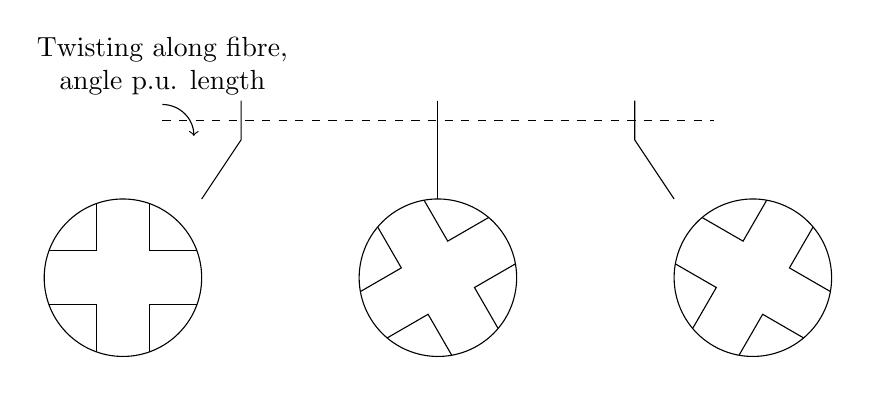
\begin{tikzpicture}
		\Tube{4mm}{25}{white}{black}{(0,0) to[out=0,in=180] (5,0)}
		\draw (0,0.25) -- (0,-0.25) -> (-0.5, -1);
		\draw (2.5,0.25) -- (2.5,-0.25) -> (2.5, -1);
		\draw (5,0.25) -- (5,-0.25) -> (5.5,-1);
		%first, non-rotated cross
		\draw (-1.5,-2) circle (1);
		\draw (-0.56,-1.66) -- (-1.16,-1.66) -- (-1.16,-1.06);
		\draw (-1.84,-1.06) -- (-1.84,-1.66) -- (-2.44,-1.66);
		\draw (-2.44,-2.34) -- (-1.84,-2.34) -- (-1.84,-2.94);
		\draw (-1.16,-2.94) -- (-1.16,-2.34) -- (-0.56,-2.34);
		%second rotated scross
		\begin{scope}[rotate around={30:(2.5,-2)}]
			\draw (2.5,-2) circle (1);
			\draw (4-0.56,-1.66) -- (4-1.16,-1.66) -- (4-1.16,-1.06);
			\draw (4-1.84,-1.06) -- (4-1.84,-1.66) -- (4-2.44,-1.66);
			\draw (4-2.44,-2.34) -- (4-1.84,-2.34) -- (4-1.84,-2.94);
			\draw (4-1.16,-2.94) -- (4-1.16,-2.34) -- (4-0.56,-2.34);			
		\end{scope} 
		%final rotated scross
		\begin{scope}[rotate around={60:(6.5,-2)}]
			\draw (6.5,-2) circle (1);
			\draw (8-0.56,-1.66) -- (8-1.16,-1.66) -- (8-1.16,-1.06);
			\draw (8-1.84,-1.06) -- (8-1.84,-1.66) -- (8-2.44,-1.66);
			\draw (8-2.44,-2.34) -- (8-1.84,-2.34) -- (8-1.84,-2.94);
			\draw (8-1.16,-2.94) -- (8-1.16,-2.34) -- (8-0.56,-2.34);			
		\end{scope} 
		%axial line and twisting arrow
		\draw[dashed] (-1,0) -- (6,0);
		\draw[->] (-1,0.2) arc (90:0:0.4);
		\node[anchor=south, align=center] at (-1,0.2) {Twisting along fibre, \\ angle p.u. length};
	\end{tikzpicture}
	\caption{Illustration of the extension into 3 dimensions, assuming a twist in the fibre. The $\bracs{x,y}$-plane's structure is rotated through some angle per unit length, represented schematically by the unit cells shown below the fibre. \label{fig:TwistedFibres}}
\end{figure}
Additionally one of the key features of optical fibres is that they can direct light around corners; and in order for PCFs to compete with optical fibres they need to offer this feature as well.
This offers another 3-dimensional system to consider; in this the fibre is not parallel to the $z$-axis but instead curves through some angle.
The primary concern in these problems will be to measure the optical loss along the fibre, and (particularly in the twisted fibre case) whether the geometry down the fibre has a decided effect on the spectrum, hence the operating frequencies.
To approach these problems, one may first chose to employ numerical techniques as in \cref{Homogenisation} --- the finite element method is perfectly applicable in 3-dimensions and deals with complex domain geometry.
However this does not provide us with an analytical model that can be used to explain any of the features we may observe.
For this we may turn to the previous analysis on the singular-structure problem for the $\bracs{x,y}$-geometry, a simple model could envisage the geometry along the fibre as a (curved) rectangular \say{sheet}, where the profile of the solution along the $x,y$ plane is known --- coming from the edge solution on the graph.
Clearly this runs into complications when the fibre has a twist, as we would need to deal with the rotation along the fibre with an appropriate set of co-ordinates.
However such models have the potential to provide highly informative models for the loss in PCFs, and whether they can match the desirable features of optical fibres (such as that of guiding light around corners).

\section{Closing Remarks}
This report has demonstrated some of the key concepts and methods that provide potential for a new model of PCFs which can be used to inform their design.
These models incorporate theory from quantum graphs and homogenisation theory present to obtain information about complex thin-structure problems from comparatively more accessible singular-structure problems.
In turn the information that can be gained from this model can feedback into the design process for PCFs, and also look to identify the cause-effect relationship of fibre-geometry to spectrum.
Formulations in both a 2-dimensional and 3-dimensional setting have been given and briefly discussed with the aim of motivating future study in these directions.
What is clear is that this presents an exciting method for PCFs, and reasons for extending the existing mathematical theory it is associated with.